% !TeX program = lualatex
% !TeX encoding = utf8
% !TeX spellcheck = uk_UA
% !BIB program = bibtex8

\documentclass[]{beamer}
\usetheme{QuantumChemistry}
\usepackage{QuantumChemistry}

\title[Лекції з квантової хімії]{\huge\bfseries Атом водню та воднеподібні атоми}
\subtitle{Лекції з квантової хімії}
\author{Пономаренко С. М.}
\graphicspath{{pictures/}}
\date{}
\begin{document}
%=======================================================================================================
\usebackgroundtemplate{
	\tikz\node[opacity=0.3]{\includegraphics[width=\paperwidth,height=\paperheight]{background}};%
}
\begin{frame}
    \thispagestyle{empty}
	\titlepage
%    \begin{center}
%        \includegraphics[width=0.3\linewidth]{LogoPhes}
%    \end{center}
\end{frame}
%=======================================================================================================
\usebackgroundtemplate{
}

%=======================================================================================================
%============================================================================
\begin{frame}[t]{Атом водню}{Історичні аспекти}
%---------------------------------------------------------
\begin{minipage}{0.55\linewidth}\tiny\coursive
       Первый шаг всегда труден и незаметен. Поэтому об Иоганне Якобе Бальмере (1825—1898), который впервые обнаружил какую-то систему в этом хаосе чисел, мы знаем очень мало. Известно, что родился он 1 мая 1825 года в маленьком городке Лаузене Базельского кантона, там же окончил среднюю школу, а затем изучал математику в университетах Карлсруэ, Берлина и Базеля. В 1869 году он стал доктором философии и приват-доцентом Базельского университета, но вскоре оставил профессорское кресло и предпочел преподавать физику в женской гимназии. Бальмеру было уже 60 лет, когда он вдруг заметил, что четыре спектральные линии в видимой части спектра водорода расположены не беспорядочно, а образуют серию, которую можно описать единой формулой:
\begin{equation*}\label{}
    \tcbhighmath[drop fuzzy shadow]{\lambda = b\frac{k^2}{k^2 - n^2}}
\end{equation*}
        где $n = 2$, $k = 3,4,5,6$, $b = 3645.6$~\AA.
\end{minipage}%
%---------------------------------------------------------
\begin{minipage}{0.45\linewidth}\centering
    \begin{center}
        \includegraphics[width=\linewidth]{Spectra}
    \end{center}
\end{minipage}
%---------------------------------------------------------
\begin{center}\tiny
\begin{tabular}{cccc}
{Вычисленно Бальмером} & {Измерено Ангстремом} & $n$ & $k$ \\ \hline
$6562.08$  & $6562.10$ & 2  & 3 \\
$4860.80$ & $4860.74$ & 2 & 4 \\
$4340.00$ & $4340.10$ & 2 & 5 \\
$4101.30$ & $4101.20$ & 2 & 6
\end{tabular}
\end{center}
{\tiny Цитується по книзі: По ту сторону кванта Л. Пономарев }
\end{frame}
%============================================================================
%============================================================================
\begin{frame}[t]{Атом водню}{Історичні аспекти}
%---------------------------------------------------------
\begin{center}
\begin{minipage}{0.45\linewidth}\centering
\begin{center}
    \includegraphics[width=\linewidth]{Spectra}
\end{center}
\end{minipage}%
\hfill
\begin{minipage}{0.45\linewidth}\centering
\begin{center}
Формула Рідберга
\begin{equation*}\label{}
    \tcbhighmath[drop fuzzy shadow]{\frac1\lambda = Ry \left( \frac{1}{n^2} - \frac{1}{m^2}\right)}
\end{equation*}
$Ry = 1.77576096 \cdot 10^{7}$~1/м
\end{center}
\end{minipage}
\end{center}
%---------------------------------------------------------
%---------------------------------------------------------
\begin{center}
\begin{minipage}{0.45\linewidth}\centering
\begin{center}
    \includegraphics[width=0.9\linewidth]{BohrModel}
\end{center}
\end{minipage}%
\hfill
\begin{minipage}{0.45\linewidth}\centering
\begin{center}
    \includegraphics[width=0.75\linewidth]{ExplanationSpectra}
\end{center}
\end{minipage}
\end{center}
%---------------------------------------------------------
\end{frame}
%============================================================================


%============================================================================
\begin{frame}{Рівняння Шредінґера}{Проклтые квантовые скачки}
\begin{block}{}\small\justify\coursive
Бор всегда не мог дождаться, когда проснется больной Шредингер, и будил его для продолжения дискуссий. В конце концов, изнуренный Шредингер заявил: "\emphs{Если эти проклятые квантовые скачки сохранятся в физике, я простить себе не смогу, что вообще связался с квантовой теорией!}". И Бор смягчился. Спор не разрешился, но в этой фразе проявился не научный спор, а человеческий характер. Бор: "Но зато все мы чрезвычайно благодарны Вам \ldots Ваша волновая механика принесла с собой такую математическую ясность и простоту, что явилось гигантским шагом вперед".

\medskip

Шредингер уехал в подавленном состоянии. Он не смог защитить смысл  $\Psi$-функции, Шредингер полагал, что $|\Psi|^2$ определяет плотность "распределения" частицы, размазанной по пространству.
\end{block}
\end{frame}
%============================================================================
\begin{frame}{Атом водню}{V СОЛЬВЕЕВСЬКИЙ КОНГРЕС (1927 ГОД)}
       \begin{center}
            \includegraphics[width=\linewidth]{Solwey}
        \end{center}
\begin{center}\small
МЕМ: Сумарний інтелект цих людей більше ніж у всіх разом на цій планеті
\end{center}
\end{frame}
%============================================================================

%============================================================================


\begin{frame}
	\frametitle{Рівняння Шредінґера для воднеподібного атома}
	\begin{center}
		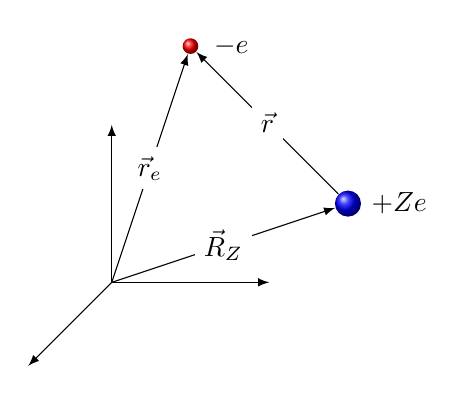
\begin{tikzpicture}
            \draw[-latex] (0,0) -- ++(2,0);
            \draw[-latex] (0,0) -- ++(0,2);
            \draw[-latex] (0,0) -- (225:1.5);
            \node[circle, ball color=red, inner sep=2pt] (e) at (1,3) {}; \node[right=5pt] at (e) {$-e$};
            \node[circle, ball color=blue] (Z) at (3,1) {}; \node[below, right=5pt] at (Z) {$+Ze$};
            \draw[-latex] (0,0) -- node[fill=white] {$\vec{R}_Z$} (Z);
            \draw[-latex] (0,0) -- node[fill=white] {$\vec{r}_e$} (e);
            \draw[-latex] (Z) -- node[fill=white] {$\vec{r}$} (e);
        \end{tikzpicture}
	\end{center}
	\begin{equation}\label{ShE}
		\tcbhighmath[drop fuzzy shadow]{\frac{\hbar^2}{2m_e}\frac{\partial^2 \Psi}{\partial \vec r_e^2} + \frac{\hbar ^2}{2m_Z}\frac{\partial^2 \Psi}{\partial \vec R_Z^2} + \left(E_\mathrm{tot} + \frac{Ze}{r} \right)\Psi  = 0}
	\end{equation}
	де  $\vec{r_e}$ і $\vec{R}_Z$ радіус-вектори, відповідно, електрона і ядра, $E_\mathrm{tot}$ --- повна енергія системи.
\end{frame}
%=======================================================================================================
\begin{frame}
	\frametitle{Рівняння Шредінґера для воднеподібного атома}
	\framesubtitle{Адіабатичне наближення}

	Хвильову функцію можна представити у вигляді:

	\begin{equation}\label{BO}
		\Psi = \psi(\vec r)\chi(\vec R)
	\end{equation}

	Рівняння Шредінгера~\eqref{ShE} дозволяє розділити змінні.

	\begin{equation}\label{key}
		\frac{\hbar ^2}{2(m_e + m_z)} \cdot \frac{\partial ^2\chi(\vec R)}{\partial \vec R^2} + E_\mathrm{CM}\cdot\chi(\vec R) = 0
	\end{equation}
	--- описує рівномірний прямолінійний рух центру мас, а рівняння
	\begin{equation}\label{ShE_relative}
		\frac{\hbar ^2}{2m}\frac{\partial ^2\psi(\vec r)}{\partial \vec r^2} + \left( E + \frac{Ze^2}{r} \right)\psi(\vec r) = 0
	\end{equation}
	--- рівняння для відносного руху, де $m\approx m_e$~--- приведена маса, $E_\mathrm{tot} = E_\mathrm{CM} + E$~--- повна енергія системи.

\end{frame}

\begin{frame}
	\frametitle{Атомні одиниці}

\begin{overprint}
\onslide<1>
\begin{block}{Атомна система одиниць}\small
одна з природних систем одиниць, яка застосовується в атомній фізиці та квантовій хімії, де в розрахунках часто використовується заряд і маса електрона. Вперше запропонована Д. Хартрі в 1928 році. Стандартне позначення англ. Atomic Units (au або a.u.)
\end{block}
\onslide<2>
\begin{center}
\alert{Рівняння Шредінгера для електрона в полі ядра}
\end{center}
\begin{equation*}\label{ShEdimless}
	\tcbhighmath{\left( -\frac12\nabla^2 - \frac{Z}{r}\right) \Psi = E\psi,}
\end{equation*}
\end{overprint}

\bigskip

Борівський радіус: $a_0  = \frac{\hbar^2}{me^2} \approx 0.53$~\AA.

Одиниця енергії $E_0 = \frac{e^2}{a_0} = -\frac{me^4}{\hbar^2} = 27.211 3845(23)$~еВ.

\begin{block}{Атомні одиниці}\small
Стала планка: $\hbar = 1$ -- атомна одиниця дії,\\
Елементарний заряд: $e=1$ -- атомна одиниця заряду,  \\
Радіус бора: $a_0 = 1$ -- атомна одиниця довжини, \\
Маса електрона: $m_{e}=1$, атомна одиниця маси.
\end{block}
%	\begin{align}\label{ucertainty}
%		r_{\min} & = \frac1Z\frac{\hbar^2}{me^2} = \frac{a_0}{Z},                                     \\
%		E_{\min} & = E(a_0) = -\frac12\left( \frac{mZ^2e^4}{\hbar^2}\right) = - \frac{ZE_0}{2},
%	\end{align}
\end{frame}
\begin{frame}
	\frametitle{Радіальна та кутова частини}
	Сферичні координати:
	\begin{center}
		\includegraphics[width=0.5\linewidth]{SphericalCoords}
	\end{center}

	$\nabla^2$~--- лапласіан в безрозмірних координатах, з якого можна виділити радіальну та кутову частину в сферичних координатах
	\begin{equation}\label{key}
		\nabla^2 =
		\underbrace{
			\frac{1}{r^2} \frac{\partial}{\partial r} r^2 \frac{\partial}{\partial r}
			}_{\text{радіальна частина} = \nabla^2}
		+ \quad
		\frac{1}{r^2}
		\underbrace{
			\left(
			\frac{1}{\sin\theta} \frac{\partial }{\partial \theta}  \sin \theta \frac{\partial}{\partial \theta} + \frac{1}{\sin^2\theta}\frac{\partial^2}{\partial \varphi^2}
			\right)
			}_{\text{кутова частина} = - \hat L^2}.
	\end{equation}
\end{frame}

\begin{frame}{Безрозмірне рівняння}{Розділення змінних}
\begin{equation*}\label{ShEdimless}
	\tcbhighmath{\left( -\frac12\nabla^2 - \frac{Z}{r}\right) \Psi = E\psi,}
\end{equation*}
	Радіальну частину лапласіана позначимо як $\nabla^2_{r}$, а кутову $ -\hat L^2$, отже:
	\begin{equation}\label{ShEdimlessSpherical}
		\left[ -\frac{\nabla_{r}^2}{2} + \frac{\hat L^2}{2r^2}  - \frac{Z}{r}\right] \psi = E\psi,
	\end{equation}

	Як відомо, рівняння \eqref{ShEdimlessSpherical} дозволяє розділити змінні, представивши хвильову функцію у вигляді добутку радіальної та кутової частини:
	\begin{equation}\label{Psi}
		\psi (r,\theta,\phi) = R(r) \cdot Y(\theta,\phi ).
	\end{equation}
\end{frame}

\begin{frame}{Аналіз кутової частини}{}
	\only<1-2,4-5>{
		Функції $Y(\theta, \psi)$ є власними функціями оператора $\hat L^2$:
		\begin{equation}
			\hat L^2 Y_l^m(\theta,\phi) = l(l+1)Y_l^m(\theta,\phi) \label{AngularMomentum},
		\end{equation}
		з власними значеннями:
		\begin{equation}
			L^2 = l(l+1).
		\end{equation}
	}

	\only<1>{
		Функції $Y_l^m(\theta,\phi )$~--- називаються сферичними функціями (або сферичними гармоніками)  і мають вигляд:
		\begin{equation}\label{SpherHarmonics}
			Y_l^m(\theta,\phi ) = \sqrt{\frac{2l+1}{4\pi} \frac{(l-|m|)!}{(l+|m|)!}} P_l^{|m|}(\cos\theta)e^{im\phi},
		\end{equation}
		де \(P_l^{|m|}(\cos\theta)\)~--- приєднані поліноми Лежандра ($x = \cos\theta$):
		\begin{equation}\label{Legandre}
			P_l^{|m|}(\cos\theta) = \frac{1}{2^ll!}(1-x^2)^{\frac{|m|}{2}}\frac{d^{l+|m|}}{dx^{l+|m|}}(x^2-1)^l.
		\end{equation}
	}

	\only<2>{

		Сферичні функції нормовані умовою:
		\begin{equation*}
			\int\limits_{0}^{\pi}\int\limits_{0}^{2\pi}|Y_l^m|^2\sin\theta d\theta d\phi = 1.
		\end{equation*}
	}

	\only<3>{
		Явний вигляд кількох сферичних гармонік наведений в таблиці.
		\begin{table}[htbp!]\small
%			\caption{Сферичні гармоніки \label{tabl:SpherHarm}}
            \begin{tblr}{
                colspec={X[l, m]X[l, m]X},
                rowsep = 0pt,
                row{1} = {l, bg=cyan!50}
            }
            \toprule
            $l$ & $m$     & $Y_l^m(\theta,\phi)$                                           \\
            \midrule
            $0$ & $0$     & $\sqrt{\frac{1}{4\pi}}$                                     \\
            \midrule
            $1$ & $0$     & $\sqrt{\frac{3}{4\pi}} \cos\theta$                          \\
            $1$ & $1$     & $-\sqrt{\frac{3}{8\pi}} \sin\theta \, e^{i\phi}  $           \\
            $1$ & $-1$    & $\sqrt{\frac{3}{8\pi}} \sin\theta \, e^{-i\phi}    $         \\
            \midrule
            $2$ & $0$     &$ \sqrt{\frac{5}{16\pi}} (3 \cos^2\theta - 1)    $            \\
            $2$ & $1$     &$ -\sqrt{\frac{15}{8\pi}} \sin\theta \cos\theta \, e^{i\phi} $\\
            $2$ & $-1$    &$ \sqrt{\frac{15}{8\pi}} \sin\theta \cos\theta \, e^{-i\phi} $\\
            $2$ & $2$     &$ \sqrt{\frac{15}{32\pi}} \sin^2\theta \, e^{2 i\phi}       $\\
            $2$ & $-2$    &$ \sqrt{\frac{15}{32\pi}} \sin^2\theta \, e^{-2 i\phi}      $\\
            \bottomrule
            \end{tblr}
		\end{table}
	}

	\only<4>{
		Оператор $\hat L$~--- є оператором моменту імпульсу (виражений в одиницях $\hbar$), а рівняння~\eqref{AngularMomentum} є рівнянням на власні значення та власні функції оператора квадрата моменту імпульсу.

		Квантове число $l$ визначає модуль момента імпульсу. Стани з значеннями $l$ позначають літерами латинського алфавіту:

		\begin{table}[htbp!]
			\begin{tabularx}{1\textwidth}{l*5{>{\centering\arraybackslash}X}}
				\toprule
				\rowcolor{cyan!40}
				Значення $l$ & 0   & 1   & 2   & 3   & 4   \\ \midrule
				Позначення & $s$ & $p$ & $d$ & $f$ & $g$ \\ \bottomrule
			\end{tabularx}
		\end{table}

	}

	\only<5>{
		Сферичні гармоніки є також власними функціями оператору проекції моменту імпульсу $L_z$ (вираженого в одиницях $\hbar$) на вісь $z$:
		\begin{equation}
			\hat L_z Y(\theta, \phi) = m  Y(\theta, \phi)
		\end{equation}

		З рівняння~\eqref{SpherHarmonics} випливає, що стани з заданим моментом імпульсу та його проекцією можливі, якщо $l \ge |m|$. З фізичної точки зору це означає, що проекція по модулю не може перевищувати сам вектор, тому можливі значення квантового числа $m$:
		\begin{equation}
			m = 0, \pm 1, \pm 2, \ldots, \pm l.
		\end{equation}
	}

	\only<6>{
		%Повне число функцій, які відповідають даному значенню $l$, дорівнює $2l + 1$.

		Комутатор операторів \(\left[ \hat L^2, \hat L_z \right] =  0 \), а комутатори $\left[ \hat L_x, \hat L_z\right] \neq 0 $ та  $\left[ \hat L_y, \hat L_z\right] \neq 0 $, це означає що одночасно можуть бути визначеними лише абсолютне значення моменту імпульсу і його проекція на вісь $z$, дві інші проекції є невизначеними. Отже, $\vec L$ перцесує навколо осі $z$ описуючи конуси з вершиною в початку координат.
		\begin{figure}[tbph!]
			\centering
			\includegraphics[width=0.8\linewidth]{SpaceQuantiz}
			\caption{Просторове квантування}
			\label{fig:spacequantiz}
		\end{figure}
	}
\end{frame}

%\begin{frame}
%	\frametitle{Розв'язки рівняння}
%
%	\only<1>
%	{
%		Сферичні координати:
%		\begin{center}
%			\includegraphics[width=0.5\linewidth]{SphericalCoords}
%		\end{center}
%	}
%	\only<1-2>
%	{
%		\begin{align}
%			\frac{1}{r^2}\frac{\partial}{\partial r} \left( r^2\frac{\partial\psi}{\partial r} \right)
%			+ \frac{1}{r^2\sin^2\theta} \frac{\partial^2\psi}{\partial\varphi^2}
%			  & + \frac{1}{r^2\sin\theta} \frac{\partial}{\partial\theta} \left( \sin\theta \frac{\partial\psi}{\partial\theta} \right) + \nonumber \\
%			  & + \frac{2m}{\hbar^2} \left( E+\frac{Ze^2}{r} \right) \psi = 0.
%		\end{align}
%	}
%	\only<2>
%	{
%		Розв'язки шукають у вигляді:
%		\begin{equation}
%			\psi(r,\theta,\varphi) = R(r)Y(\theta, \varphi ).
%		\end{equation}
%	}
%	\only<3>
%	{
%		\begin{equation*}
%			\psi_{nlm}(r,\theta,\varphi) = R_{n,l}(r)Y_{l,m}(\theta, \varphi )
%		\end{equation*}
%		\begin{center}
%			де
%		\end{center}
%
%		\hrulefill	 \raisebox{-0.2\baselineskip}{ Радіальна частина } \hrulefill
%
%		\(
%		R_{n,l}(r) = \frac{1}{\sqrt{2n {\cdot} (n-l-1)! {\cdot} (n+l)!} } {\cdot} {\left (  \frac{2Z}{n a_0} \right )}^{\frac32} \exp{ \left( {- \frac{Zr}{n a_0}} \right) } {\cdot} {\left( \frac{2rZ}{n a_0} \right)}^{l} L_{n-l-1}^{2l+1}{ \left( \frac{2rZ}{n a_0} \right)}
%		\),
%
%		$a_0$ --- борівський радіус,\\
%		$L_{n-l-1}^{2l+1}{\left(\frac{2rZ}{n a_0}\right)}$ --- узагальнені поліноми Лагерра степені $n-l-1$ від аргумента $\frac{2r}{n a_0}$,\\
%		\hrulefill	 \raisebox{-0.2\baselineskip}{ Кутова частина } \hrulefill
%
%		$Y_{l,m}=  (-1)^m \sqrt{\frac{2l+1}{2} \frac{(l-m)!}{(l+m)!}} P^m_l (\cos\theta) \times \frac{1}{\sqrt{2 \pi}} e^{i m \varphi}$ --- сферичні функції,\\
%		$P^m_l (\cos\theta)$ --- приєднані поліноми Лежандра.
%	}
%
%\end{frame}
%=======================================================================================================
%\begin{frame}
%	\frametitle{Квантові числа $n$, $l$, $m$, та їх фізичний зміст}
%	\begin{tabular}{|c|c|c|}
%		\hline
%		Енергія електрона                              & Момент імпульсу & Проекція моменту імпульсу \\
%		\hline
%		$E_n = -\frac{1}{n^2} \frac{m_e Z^2e^4}{8h^2 \varepsilon_0^2}$ & $L = \sqrt{l(l+1)}\hbar$      & $L_z = m\hbar$                                   \\
%		\hline
%	\end{tabular}
%
%	\begin{center}
%		Просторове квантування:
%
%		\includegraphics[width=0.4\linewidth]{SpaceQuantizing}\hfil
%		\includegraphics[width=0.4\linewidth]{SpaceQuantizing2}
%	\end{center}
%
%	\begin{tabular}{|l|c|}
%		\hline
%		Головне квантове число       & $n = 1,2,3,4,5,\ldots $                \\
%		\hline
%		Орбітальне квантове число & $l = 0,1,\ldots, n-1$                  \\
%		\hline
%		Магнітне квантове число     & $m = -l,\ldots,0,\ldots, l$            \\
%		\hline
%		Кратність виродження          & $\sum\limits_{l=0}^{n-1} (2l+1) = n^2$ \\
%		\hline
%	\end{tabular}
%
%\end{frame}

\begin{frame}{Аналіз кутової частини}{Декартовий базис}
	\only<1>{
		Гармоніка $Y_{1,0}$  є дійсною функцією косинуса. Косинус має максимальну величину при $\theta = 0$ і $\theta = \pi$, що співпадає з напрямком осі $OZ$ декартової системи координат, тому цю функцію зручно назвати $p_z$, виразивши її через декартову координату $z$:
		\begin{equation*}
			Y_{1}^0 = \sqrt{\frac{3}{4\pi}} \cos\theta = \sqrt{\frac{3}{4\pi}} \frac{z}{r} = p_z,
		\end{equation*}
		оскільки $z = r\cos\theta$. Однак дві інші функції, які відповідають тому ж самому орбітальному числу $l = 2$, мають складний вираз, кожна з яких містить уявний компонент $e^{im\phi}$ і не відповідає якомусь визначеному напрямку.
	}
	\only<2>{\small
		\begin{tblr}{
            colspec={X[l, m]X[l, m]X[l, m]},
            row{1} = {c, m, bg=cyan!50},
        }
        \toprule
        Назва стану & Суперпозиція & Значення \\
        \midrule
        $p_x$ & $\frac{1}{\sqrt{2}} \left( Y_1^{-1} - Y_1^{+1} \right)$ & $\sqrt{\frac{3}{4\pi}} \frac{x}{r}$ \\
        $p_y$ & $\frac{i}{\sqrt{2}} \left( Y_1^{-1} + Y_1^{+1} \right)$ & $\sqrt{\frac{3}{4\pi}} \frac{y}{r}$ \\
        $p_z$ & $Y_1^0$ & $\sqrt{\frac{3}{4\pi}} \frac{z}{r}$ \\
        \midrule
        $d_{x^2 - y^2}$ & $\frac{1}{\sqrt{2}} \left( Y_2^{+2} + Y_2^{-2}\right)$ & $\sqrt{\frac{15}{16\pi}} \frac{x^2 - y^2}{r^2}$ \\
        $d_{xy}$ & $\frac{-i}{\sqrt{2}} \left( Y_2^{+2} - Y_2^{-2}\right)$ & $\sqrt{\frac{15}{16\pi}} \frac{xy}{r^2}$ \\
        $d_{xz}$ & $\frac{-1}{\sqrt{2}} \left( Y_2^{+1} - Y_2^{-1}\right)$ & $\sqrt{\frac{15}{16\pi}} \frac{xz}{r^2}$ \\
        $d_{yz}$ & $\frac{i}{\sqrt{2}} \left( Y_2^{+1} + Y_2^{-1}\right)$ & $\sqrt{\frac{15}{16\pi}} \frac{yz}{r^2}$ \\
        $d_{z^2}$ & $Y_2^0$ & $\sqrt{\frac{5}{16\pi}} \frac{3z^2 - r^2}{r^2}$ \\
        \bottomrule
		\end{tblr}
	}

	\only<3>{%
\begin{columns}
	\begin{column}{0.5\linewidth}
         \begin{center}
            \includegraphics[width=1\linewidth]{Nodal}
        \end{center}
	\end{column}
	\begin{column}{0.5\linewidth}
 		\begin{center}
			\includegraphics[width=\linewidth]{PORB}\\
            \includegraphics[width=1\linewidth]{DORB}
		\end{center}
	\end{column}
\end{columns}
	}
\end{frame}


\begin{frame}{Аналіз радіальної частини}

	\only<1>{
		Після підстановки~\eqref{Psi} в \eqref{ShEdimlessSpherical}врахувавши ~\eqref{AngularMomentum}, отримаємо:

		\begin{equation}\label{RadialShE}
			\left( \nabla^2_{r} - \frac{l(l+1)}{ r^2} + \frac{2Z}{r} + 2E \right) R(r) = 0
		\end{equation}


		Рівняння~\eqref{RadialShE} має розв'язки:
		\begin{equation}\label{PsiRadial}
			R_{n,l}( r) = \sqrt{\frac{4Z^3(n-l-1)!}{n^4(n+l)!}}  {\left( \frac{2Z r}{n} \right)}^{l}  L_{n-l-1}^{2l+1}{ \left( \frac{2Z r}{n} \right)} e^{- \frac{Z r}{n}}
		\end{equation}
		при значеннях
		\begin{equation}\label{EnergyDimless}
			\tcbhighmath{E = - \frac{Z^2}{2n^2},}
		\end{equation}
		де \(L_i^j(x)= \frac{x^{-j}e^x}{n!} \frac{d^i}{dx^i} \left( e^{-x} x^{i+j}\right) \)~--- узагальнений поліном Лагерра. Функції $R_{n,l}( r)$ нормовані умовою $\int\limits_{0}^{\infty} R_{n,l}^2  r^2 d r = 1$.
	}

	\only<2>{
		\def\Za{Z^{\frac32}}
		\begin{tabularx}{\textwidth}{p{0.15\linewidth}m{0.15\linewidth}*1{>{\arraybackslash}X}}
			\toprule
			\rowcolor{cyan!40}
			$n$ & $l$ & $R_{n,l}$                                                       \\ \midrule
			1   & 0   & $2                     \Za    e^{-Z r}                        $ \\ \midrule
			2   & 0   & $\dfrac{1}{2\sqrt{2}}   \Za   (2-Z r)e^{-Z r/2}               $ \\[2ex]
			2   & 1   & $\dfrac{1}{2\sqrt{6}}   \Za   Z r e^{-Z r/2}                  $ \\[2ex] \midrule
			3   & 0   & $\dfrac{2}{81\sqrt{3}}  \Za  (2Z^2 r^2 - 18Z r + 27) e^{-Z r/3}$ \\[2ex]
			3   & 1   & $\dfrac{4}{81\sqrt{6}}  \Za  (6Z r - Z^2 r^2) e^{-Z r/3}       $ \\[2ex]
			3   & 2   & $\dfrac{4}{81\sqrt{30}} \Za  Z r^2 e^{-Z r/3}                 $ \\ \bottomrule
		\end{tabularx}
	}

	\only<3>{
		Вигляд радіальної залежності
		\begin{center}
			\includegraphics[width=0.9\linewidth]{RadialOrbitalDencity}
		\end{center}
	}
\end{frame}



\begin{frame}{Що таке орбіталь?}
	Орбіталь --- одноелектронна хвильова функція, яка є розв'язком рівняння Шредінгера для воднеподібного атома; задається  головним $n$, орбітальним $l$, і магнітним $m$ --- квантовими числами.

Середні розміри атома атома задаються формулою
, яку можна отримати з співвідношення:
\begin{equation*}
	\left\langle r\right\rangle =  \int\limits_{V} \psi(r,\theta,\varphi) r \psi^*(r, \theta, \varphi) dV
\end{equation*}

\begin{equation*}
	\left\langle r \right\rangle = \frac{a_0}{Z}n^2 \left( \frac32 - \frac{l(l+1)}{2n^2}\right)
\end{equation*}


\end{frame}

\end{document}
